% ==========================================================
% CHƯƠNG 2: CƠ SỞ LÝ THUYẾT
% ==========================================================

\chapter{Cơ sở lý thuyết}
\label{ch:co_so_ly_thuyet}
\section{Tổng quan về vệ tinh nhỏ và nhu cầu mô đun thí nghiệm đa năng}
\label{sec:tong_quan_chuong2}

Vệ tinh nhỏ, đặc biệt là CubeSat, là nền tảng nghiên cứu và trình diễn công nghệ được sử dụng phổ biến trong các trường đại học, viện nghiên cứu và doanh nghiệp không gian mới. So với vệ tinh truyền thống, CubeSat có ưu điểm nổi bật là chi phí phát triển thấp hơn, thời gian thiết kế ngắn hơn và quy trình tích hợp linh hoạt hơn. Tuy nhiên, các hệ thống trên CubeSat luôn bị ràng buộc đồng thời bởi giới hạn kích thước, khối lượng, công suất và môi trường vận hành khắc nghiệt.

Trong đề tài này, luận văn không đi sâu vào mục tiêu của thí nghiệm mà tập trung vào kiến trúc điều khiển và truyền nhận dữ liệu giữa các board mạch chức năng. Cụ thể, hệ thống bao gồm board mạch EXP (Experiment board để điều khiển thí nghiệm, xử lí dữ liệu và giao tiếp người dùng), board mạch IF (Interface board để giao tiếp với các board khác và giao tiếp người dùng), thí nghiệm cụ thể được thiết kế để trực quan hóa hệ thống là hệ thí nghiệm quang học bao gồm board mạch LASER và PHOTO. Board mạch LASER (Laser diode board dùng để điều khiển tín hiệu quang), board mạch PHOTO (Photo diode board dùng để thu thập tín hiệu quang). Mục tiêu cốt lõi là xây dựng và kiểm chứng luồng điều khiển--thu thập--truyền dữ liệu cho bài toán phân tích mô hình thí nghiệm.

\subsection{Khái niệm CubeSat và phương thức triển khai quỹ đạo}
\label{subsec:khai_niem_cubesat}

Trong phạm vi luận văn, thuật ngữ vệ tinh được hiểu là vệ tinh nhân tạo, tức các hệ thống được phóng lên quỹ đạo để thực hiện nhiệm vụ cụ thể. CubeSat là một lớp vệ tinh nhỏ sử dụng triết lý thiết kế mô-đun, cho phép cấu hình linh hoạt theo mục tiêu nhiệm vụ và tài nguyên sẵn có.

Về triển khai quỹ đạo, CubeSat thường đi theo hai phương thức chính. Thứ nhất, CubeSat được đặt trong các cơ cấu chứa/phóng chuyên dụng (dispenser/deployer) gắn trên tên lửa, sau đó được tách ra quỹ đạo bằng cơ chế lò xo. Trong kịch bản này, CubeSat thường đóng vai trò tải phụ hoặc tham gia các chuyến phóng rideshare. Thứ hai, CubeSat được vận chuyển lên Trạm Vũ trụ Quốc tế (ISS), sau đó được nạp vào các hệ deployer của ISS và thả ra quỹ đạo hoạt động.

Tương tự các vệ tinh lớn, hệ CubeSat được phân tách thành hai nhóm chức năng: \textit{satellite bus} và \textit{satellite payload}. \textit{Bus} là phần hạ tầng duy trì hoạt động của vệ tinh trong suốt nhiệm vụ, thường gồm các phân hệ: kết cấu (\textit{STRU}), truyền thông (\textit{COMM}), điều khiển tư thế và quỹ đạo (\textit{AOCS}), nguồn điện (\textit{EPS}), xử lý dữ liệu trên board (\textit{OBDH}), telemetry--tracking--command (\textit{TT\&C}) và điều khiển nhiệt (\textit{TCS}). Ngược lại, \textit{payload} là cụm thiết bị trực tiếp cung cấp năng lực nhiệm vụ của vệ tinh, ví dụ cảm biến quang học đối với vệ tinh quan sát hoặc cụm anten/phát--thu đối với vệ tinh thông tin.

Với cách phân tách này, \textit{bus} không trực tiếp tạo dữ liệu nhiệm vụ nhưng quyết định độ ổn định vận hành của toàn hệ; còn \textit{payload} tạo ra dữ liệu đầu ra nhưng phụ thuộc vào \textit{bus} để được cấp nguồn, điều khiển, đồng bộ và truyền dữ liệu. Trong phạm vi đề tài, IF thuộc lớp hạ tầng điều khiển/giao tiếp, cụm LASER--PHOTO thuộc lớp tải thí nghiệm, còn EXP đóng vai trò điều phối cục bộ giữa hai lớp này và giao tiếp ra ngoài hệ thống để kết nối với người dùng hoặc hệ thống khác. Cách ánh xạ này là cơ sở để tổ chức kiến trúc kỹ thuật và xác định luồng dữ liệu trong các mục tiếp theo.

\subsection{Chuẩn kích thước CubeSat(đơn vị U)}
\label{subsec:chuan_u}

Kiến trúc CubeSat được hình thành từ năm 1999 trong khuôn khổ dự án CubeSat do GS. Jordi Puig-Suari (California Polytechnic State University) và GS. Bob Twiggs (Stanford University) khởi xướng. CubeSat sử dụng chuẩn mô-đun theo đơn vị U (Unit), trong đó 1U tương ứng với một khối lập phương xấp xỉ 10 x 10 x 10 cm. Các cấu hình lớn hơn được tạo bằng cách ghép nhiều khối 1U theo các tổ hợp khác nhau, ví dụ 2U, 3U, 6U, 8U, 12U và 16U. Chuẩn hóa theo đơn vị U có ý nghĩa kỹ thuật quan trọng vì quyết định không gian khả dụng cho mạch điện, dây dẫn, đầu nối, kết cấu cơ khí và giải pháp tản nhiệt.

Về cơ khí, CubeSat thường được thiết kế với các rail nhôm dọc theo cạnh để tương thích với cơ cấu chứa/phóng (dispenser/deployer), do đó giới hạn kích thước thường được xác định tại vùng rail. Ngoài các chuẩn phổ biến, một số cấu hình nhỏ hơn như 0.25U đã từng được sử dụng, đồng thời các cấu hình lớn hơn như 24U và 27U cũng đã được đề xuất cho các nhiệm vụ tương lai.

\begin{figure}[H]
    \centering
    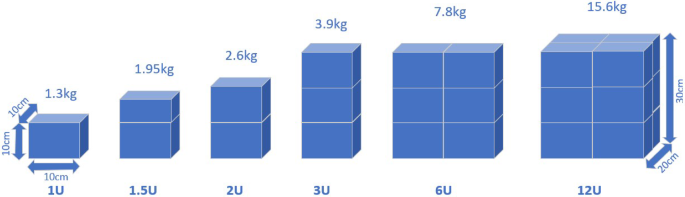
\includegraphics[width=0.85\textwidth]{picture/cube-sat-size.png}
    \caption{Kích thước chuẩn CubeSat theo đơn vị U}
    \label{fig:cubesat_size_u}
\end{figure}

\begin{table}[H]
    \centering
    \caption{Kích thước tối đa và khối lượng tối đa cho phép của CubeSat theo kích cỡ}
    \label{tab:cubesat_size_weight}
    \begin{tabular}{|c|c|c|}
        \hline
        \textbf{CubeSat Size} & \textbf{Maximum Dimensions (cm)} & \textbf{Maximum Weight (kg)} \\ \hline
        1U    & 10 x 10 x 11.35       & 2  \\ \hline
        1.5U  & 10 x 10 x 17.02       & 3  \\ \hline
        2U    & 10 x 10 x 22.70       & 4  \\ \hline
        3U    & 10 x 10 x 34.05       & 6  \\ \hline
        6U    & 22.63 x 10 x 34.05    & 12 \\ \hline
        6U XL & 22.63 x 10 x 36.60    & 12 \\ \hline
        8U    & 22.63 x 10 x 45.40    & 16 \\ \hline
        12U   & 22.63 x 22.63 x 34.05 & 24 \\ \hline
        16U   & 22.63 x 22.63 x 45.40 & 32 \\ \hline
    \end{tabular}
\end{table}

Các giá trị kích thước và khối lượng trong bảng là giới hạn điển hình theo chuẩn hình học CubeSat. Trên thực tế, giá trị cho phép cuối cùng phụ thuộc vào loại dispenser cụ thể của từng chiến dịch phóng; một số vùng có thể cho phép chi tiết nhô ra ngoài kích thước rail theo quy định kỹ thuật đi kèm.

Đối với hệ thống đề tài, ràng buộc theo chuẩn U tác động trực tiếp đến bố trí phần cứng, chiều dài liên kết, khả năng tản nhiệt và phương án kết nối dữ liệu giữa các board mạch. Việc hiểu rõ ràng buộc hình học này giúp quá trình thiết kế giao diện cơ--điện hợp lý ngay từ đầu.

\subsection{Chuẩn hóa nền tảng CubeSat và ý nghĩa thiết kế}
\label{subsec:chuan_hoa_nen_tang_cubesat}

Bên cạnh chuẩn kích thước U, hệ CubeSat còn được hưởng lợi từ nhiều mức chuẩn hóa nền tảng. Về chuẩn hóa cơ khí phóng, các cơ cấu deployer như P-POD giúp bảo đảm tương thích với nhiều phương án phóng và giảm độ phức tạp tích hợp. Về chuẩn hóa điện tử, dù chưa có một chuẩn bắt buộc duy nhất, dạng board xếp chồng theo triết lý PC/104 được sử dụng rộng rãi trong avionics CubeSat nhờ tận dụng thể tích tốt và thuận lợi cho lắp ghép mô-đun.

Ở khối nguồn, pin trụ 18650 dạng COTS thường được dùng để cấu hình bộ pin cho EPS theo hướng chi phí hợp lý và dễ thay thế linh kiện. Các mức chuẩn hóa nói trên cho thấy tư duy thiết kế CubeSat hiện đại ưu tiên tính mô-đun, tính tích hợp nhanh và khả năng kế thừa giữa các phiên bản hệ thống.

\subsection{Chuẩn giao tiếp dữ liệu và nhu cầu mô đun thí nghiệm đa năng}
\label{subsec:nhu_cau_module_da_nang}

Trong khối truyền thông nội bộ, CubeSat thường sử dụng các giao thức chuẩn như SPI, CAN Bus, I2C, UART, SpaceWire và Ethernet để liên kết các phân hệ. Việc lựa chọn giao thức phụ thuộc vào băng thông yêu cầu, độ phức tạp triển khai, khả năng chống nhiễu và mức độ mở rộng hệ thống. Cách tiếp cận theo giao thức chuẩn giúp giảm rủi ro tích hợp, tăng khả năng tương thích giữa các board mạch và thuận lợi cho quá trình kiểm thử.

Nhiều nhiệm vụ CubeSat hiện nay yêu cầu tải thí nghiệm có khả năng cấu hình linh hoạt để phục vụ nhiều kịch bản đo khác nhau. Điều này dẫn đến nhu cầu phát triển các mô đun đa năng theo hướng ``một kiến trúc, nhiều chế độ vận hành''. Với hướng tiếp cận này, hệ thống có thể tiết kiệm thời gian phát triển, giảm chi phí tạo mẫu và tăng khả năng kế thừa cho các phiên bản sau.

\section{Cơ sở lý thuyết kiến trúc hệ thống EXP--IF--LASER--PHOTO}
\label{sec:kien_truc_exp_if_photo_laser}

Hệ thống được mô hình hóa theo cấu trúc điều khiển phân cấp. EXP là board điều khiển trung tâm của hệ thống, đồng thời tích hợp hai lớp xử lý trên cùng một phần cứng. Trong đó, core MPU đảm nhiệm vai trò giao tiếp cấp cao, tiếp nhận lệnh từ người dùng, xử lý dữ liệu và quản lý trạng thái hệ thống. Core MCU chịu trách nhiệm điều khiển thí nghiệm theo thời gian thực, trực tiếp phát lệnh đến board LASER, thu dữ liệu từ board PHOTO và điều phối các phần tử chấp hành như TEC, HEATER. IF là lớp trung gian giao tiếp, có nhiệm vụ chuẩn hóa kết nối và cung cấp khả năng mở rộng interface.

\subsection{Vai trò board EXP}
\label{subsec:vai_tro_exp}

Board EXP là thành phần cốt lõi của hệ thống. EXP chịu trách nhiệm thực thi quy trình thí nghiệm, điều khiển trình tự hoạt động của LASER và PHOTO theo kịch bản định trước, đồng bộ thời điểm phát/thu tín hiệu và giám sát trạng thái thực thi. Bên cạnh đó, board còn thu thập dữ liệu từ các cảm biến môi trường như NTC, đồng thời trực tiếp điều khiển nhiệt độ buồng thí nghiệm qua TEC và HEATER. Với kiến trúc hai core, MPU trên EXP đảm nhiệm lớp xử lý và giao tiếp cấp hệ thống, còn MCU đảm nhiệm lớp điều khiển cục bộ thời gian thực. EXP cũng là nơi tổng hợp, xử lý sơ bộ, đóng gói dữ liệu theo khung truyền và gửi ra giao diện ngoài hệ thống.

\subsection{Vai trò board IF}
\label{subsec:vai_tro_if}

Board IF (Interface board) là lớp giao tiếp mở rộng của hệ thống, kết nối EXP với các giao diện ngoài và các thành phần phần cứng bổ sung tùy cấu hình triển khai. IF giúp chuẩn hóa tín hiệu điện, tổ chức đầu nối và đơn giản hóa kiến trúc dây nối nội bộ.

\subsection{Vai trò board LASER}
\label{subsec:vai_tro_laser}

Board LASER là khối phát tín hiệu quang của hệ thống thí nghiệm. Board này nhận lệnh điều khiển từ EXP để lựa chọn kênh phát, thiết lập mức kích thích và tạo ra tín hiệu quang theo cấu hình đo đã đặt trước. Vai trò chính của LASER là cung cấp nguồn kích thích quang ổn định, có khả năng điều chỉnh theo từng chế độ vận hành nhằm bảo đảm điều kiện vào nhất quán cho quá trình thí nghiệm. Chất lượng hoạt động của board LASER ảnh hưởng trực tiếp đến độ lặp lại và độ tin cậy của tín hiệu thu được ở phía PHOTO.

\subsection{Vai trò board PHOTO}
\label{subsec:vai_tro_photo}

Board PHOTO là khối thu nhận tín hiệu quang của hệ thống. Board này tiếp nhận tín hiệu ánh sáng sau khi tương tác với mẫu thí nghiệm, thực hiện các bước chuyển đổi và điều hòa tín hiệu cần thiết trước khi gửi dữ liệu về EXP để xử lý tiếp. Vai trò của PHOTO là bảo đảm tín hiệu quang thu được được chuyển thành tín hiệu điện có độ chính xác và độ ổn định phù hợp cho quá trình số hóa, từ đó phục vụ việc phân tích, đánh giá và so sánh kết quả thí nghiệm. Cùng với board LASER, board PHOTO tạo thành cặp khối chức năng trung tâm của tải thí nghiệm quang.

\section{Cơ sở lý thuyết các linh kiện}

\subsection{Cấu tạo và nguyên lý hoạt động của TEC}

\begin{figure}[H]
    \centering
    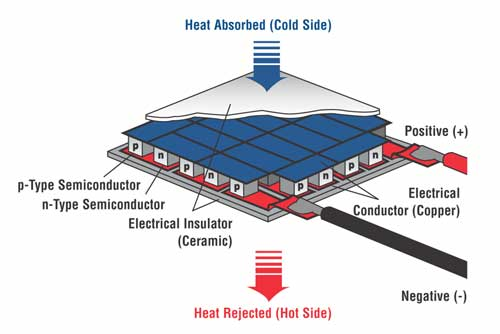
\includegraphics[width=0.7\textwidth]{picture/components/TEC.jpg}
    \caption{Linh kiện TEC}
    \label{fig:tec_module}
\end{figure}

TEC (Thermoelectric Cooler) là phần tử bơm nhiệt rắn, hoạt động dựa trên hiệu ứng nhiệt điện. Một mô-đun TEC điển hình gồm nhiều cặp bán dẫn loại p và loại n mắc điện nối tiếp, nhiệt song song; các cặp này được kẹp giữa hai tấm gốm cách điện (thường là alumina) để vừa cách điện vừa truyền nhiệt tốt. Các thanh dẫn kim loại mỏng liên kết các cặp p-n theo dạng ziczac, tạo thành một khối phẳng gọn nhẹ, không có bộ phận chuyển động cơ khí.

Hiệu ứng Peltier mô tả hiện tượng hấp thụ hoặc giải phóng nhiệt tại mối nối của hai vật liệu khác nhau khi có dòng điện một chiều đi qua. Trong TEC, khi dòng điện chạy theo một chiều xác định, các hạt tải điện mang năng lượng nhiệt từ một mặt sang mặt còn lại: một mặt sẽ hấp thụ nhiệt (mặt lạnh), mặt kia sẽ thải nhiệt (mặt nóng). Nếu đảo chiều dòng điện, vai trò hai mặt cũng đảo ngược.

Từ đó, nguyên lý hoạt động của TEC có thể hiểu là quá trình bơm nhiệt chủ động: cấp dòng DC để chuyển nhiệt từ buồng cần làm mát sang phía tản nhiệt. Nhiệt độ thực tế đạt được phụ thuộc vào dòng điều khiển, chênh lệch nhiệt độ hai mặt, khả năng tản nhiệt phía nóng và tải nhiệt của hệ thống. Vì vậy trong ứng dụng thực tế, TEC thường đi kèm khối tản nhiệt/quạt và mạch điều khiển (PWM hoặc điều khiển dòng) để ổn định nhiệt độ theo giá trị đặt.

\subsection{Cấu tạo và nguyên lý hoạt động của HEATER}

\begin{figure}[H]
    \centering
    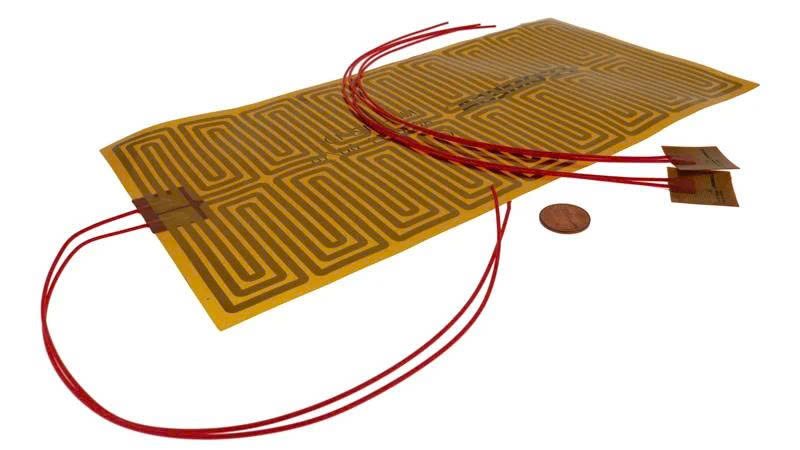
\includegraphics[width=0.5\textwidth]{picture/components/HEATER.jpg}
    \caption{Linh kiện HEATER}
    \label{fig:heater_module}
\end{figure}

HEATER là phần tử chuyển đổi điện năng thành nhiệt năng để nâng và duy trì nhiệt độ cho buồng thí nghiệm. Trong các hệ thống nhúng, HEATER thường có cấu tạo dạng điện trở công suất (resistive heater), gồm vật liệu điện trở và lớp cách điện/cách nhiệt phù hợp để truyền nhiệt hiệu quả nhưng vẫn bảo đảm an toàn điện.

Nguyên lý vật lý của HEATER dựa trên hiệu ứng Joule: khi dòng điện đi qua phần tử điện trở, công suất nhiệt sinh ra được xác định gần đúng theo biểu thức $P = I^2R$ (hoặc $P = \frac{V^2}{R}$ với nguồn áp ổn định). Nhiệt lượng này được truyền từ bề mặt HEATER sang môi trường hoặc khối vật liệu cần gia nhiệt thông qua dẫn nhiệt, đối lưu và bức xạ.

Từ đó, nguyên lý hoạt động của HEATER trong hệ thống điều khiển nhiệt là cấp công suất theo nhu cầu tải nhiệt: tăng công suất khi nhiệt độ đo được thấp hơn giá trị đặt và giảm/ngắt khi tiến gần ngưỡng yêu cầu. Trên thực tế, HEATER thường được điều khiển qua MOSFET bằng PWM hoặc điều khiển on-off theo phản hồi cảm biến nhiệt (ví dụ NTC), nhằm giữ nhiệt độ ổn định, giảm dao động và tối ưu tiêu thụ năng lượng.

\subsection{Cấu tạo và nguyên lý hoạt động của SOLENOID}

\begin{figure}[H]
    \centering
    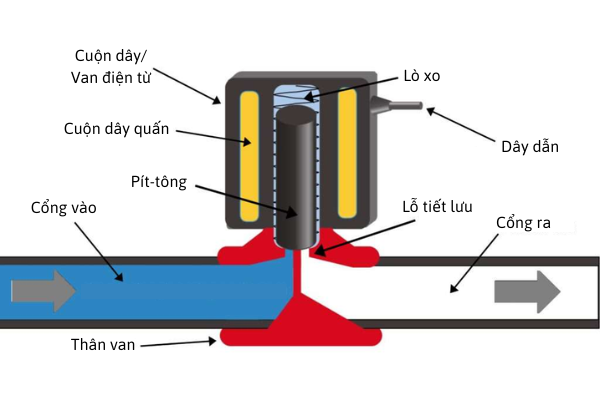
\includegraphics[width=0.7\textwidth]{picture/components/SOLENOID.png}
    \caption{Linh kiện SOLENOID}
    \label{fig:solenoid_module}
\end{figure}

SOLENOID là cơ cấu chấp hành điện từ dùng để tạo chuyển động tịnh tiến ngắn, thường phục vụ đóng/mở van, chốt cơ khí hoặc kích hoạt cơ cấu đẩy-kéo. Về cấu tạo, solenoid gồm cuộn dây dẫn quấn quanh lõi từ, vỏ dẫn từ, phần ứng (plunger) có thể di chuyển và lò xo hồi vị. Khi không cấp điện, lò xo giữ phần ứng ở vị trí ban đầu.

Nguyên lý vật lý của solenoid dựa trên từ trường sinh ra bởi dòng điện chạy qua cuộn dây. Dòng điện tạo ra từ thông trong mạch từ, sinh lực điện từ hút phần ứng về phía lõi, từ đó biến đổi năng lượng điện thành chuyển động cơ. Khi ngắt điện, từ trường suy giảm, lực hút mất đi và lò xo đưa phần ứng trở về trạng thái nghỉ.

Từ đó, nguyên lý hoạt động của SOLENOID trong hệ thống là điều khiển trạng thái cơ cấu theo tín hiệu điện: cấp điện để tác động (hút/kéo hoặc đẩy tùy cấu hình) và ngắt điện để hồi vị. Trong thực tế, solenoid thường được điều khiển qua mạch công suất MOSFET kèm diode dập xung ngược (flyback diode) để bảo vệ linh kiện chuyển mạch khỏi xung điện áp cảm ứng khi cuộn dây bị ngắt dòng.

\subsection{Tổng quan linh kiện Laser Diode}
\label{subsec:tong-quan-laser-diode}

\begin{figure}[H]
    \centering
    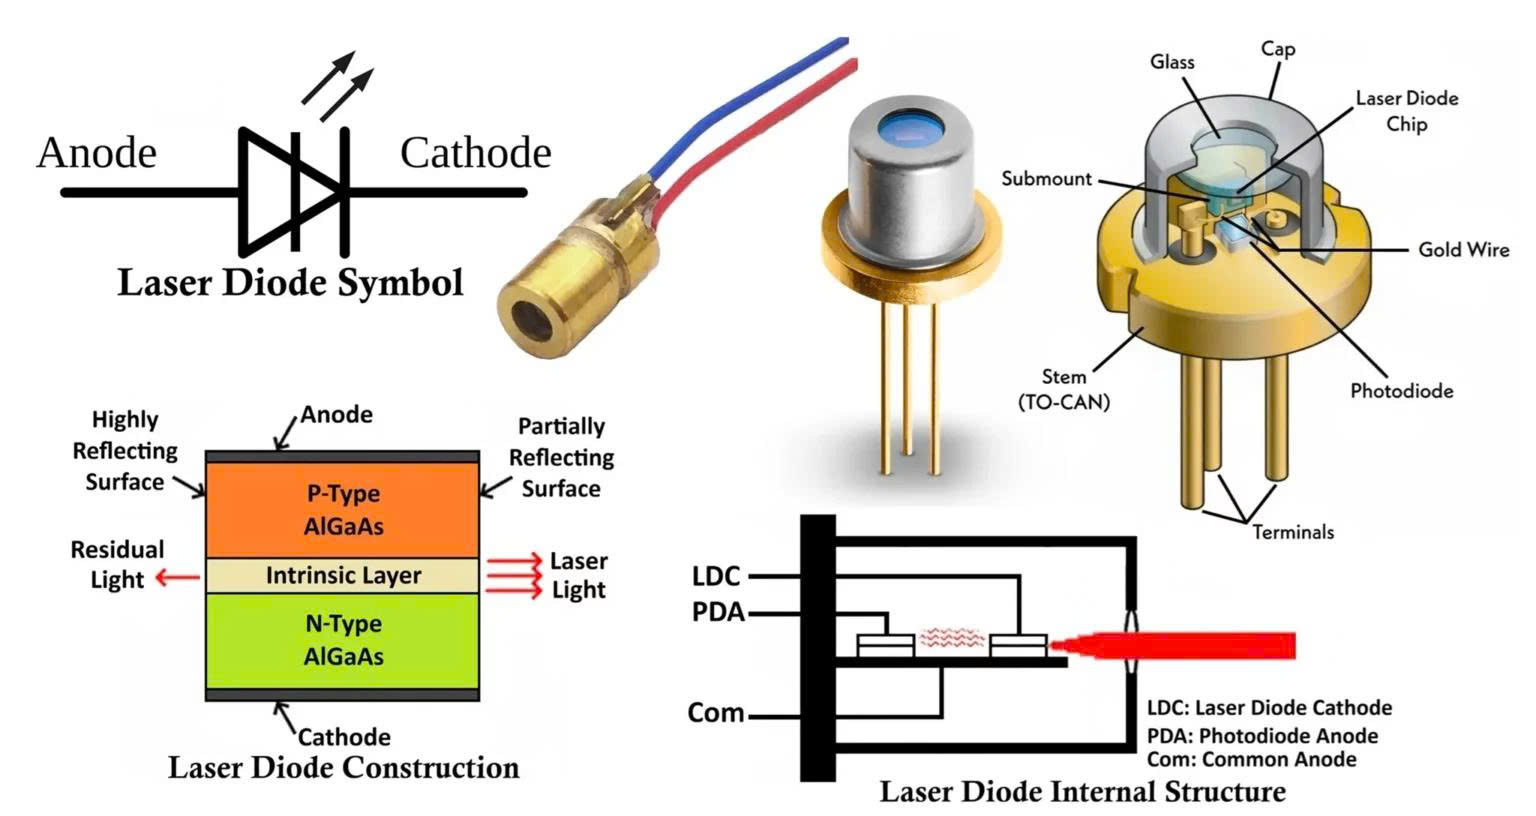
\includegraphics[width=0.8\textwidth]{picture/components/laser-diode.jpg}
    \caption{Linh kiện laser diode}
    \label{fig:component-laser-diode}
\end{figure}

Laser diode là nguồn phát quang bán dẫn hoạt động dựa trên hiện tượng phát xạ kích thích trong vùng tiếp giáp p-n. Khi phân cực thuận đủ lớn, hạt tải được bơm vào vùng hoạt tính và tạo nghịch đảo mật độ hạt. Photon sinh ra trong quá trình tái hợp sẽ kích thích các chuyển mức tiếp theo, từ đó tạo chùm sáng có tính định hướng cao, phổ hẹp và công suất quang ổn định hơn so với LED thông thường.

Về nguyên lý hoạt động, dòng điều khiển tăng đến ngưỡng sẽ đưa linh kiện vào chế độ phát laser. Dưới ngưỡng, linh kiện chủ yếu phát xạ tự phát (ánh sáng yếu, độ kết hợp thấp); trên ngưỡng, phát xạ kích thích chiếm ưu thế và công suất quang tăng nhanh theo dòng lái. Trong thiết kế thực tế, laser diode thường được điều khiển bằng mạch nguồn dòng hằng để ổn định công suất phát và hạn chế trôi do nhiệt.

Một số thông số kỹ thuật cơ bản cần quan tâm gồm: bước sóng danh định (nm), dòng ngưỡng, dải dòng làm việc, điện áp thuận, công suất quang đầu ra, góc phân kỳ chùm tia, hệ số trôi theo nhiệt độ và điều kiện tản nhiệt. Các tham số này quyết định khả năng ghép quang, mức tín hiệu thu và độ ổn định của hệ đo trong quá trình vận hành.

Trong vùng làm việc trên ngưỡng, quan hệ gần đúng giữa dòng lái và công suất quang đầu ra của laser diode thường được biểu diễn theo đặc tuyến \(L\!-\!I\) bởi:
\begin{equation}
P_{opt} \approx \eta_s \left(I_F - I_{th}\right), \qquad I_F > I_{th}
\end{equation}

Nếu xét trong khoảng thời gian phát sáng \(t\), năng lượng ánh sáng phát ra có thể được tính:
\begin{equation}
E_{opt} = P_{opt}\,t \approx \eta_s \left(I_F - I_{th}\right)t
\end{equation}

Trong đó:
\begin{itemize}
    \item \(P_{opt}\) là công suất quang đầu ra của laser diode, đơn vị W. Đây là đại lượng biểu diễn tốc độ phát năng lượng ánh sáng tại đầu ra nguồn phát.
    \item \(E_{opt}\) là năng lượng ánh sáng phát ra trong khoảng thời gian xét, đơn vị J. Khi công suất quang gần như không đổi trong thời gian \(t\), năng lượng bằng công suất nhân với thời gian.
    \item \(\eta_s\) là hệ số dốc công suất quang theo dòng lái (slope efficiency), đơn vị W/A. Tham số này cho biết khi tăng thêm \(1\,A\) dòng lái trên ngưỡng thì công suất quang đầu ra tăng thêm bao nhiêu watt. Trong datasheet, đại lượng này cũng có thể được ghi dưới dạng mW/mA.
    \item \(I_F\) là dòng thuận cấp cho laser diode, đơn vị A. Đây là dòng điều khiển thực tế chạy qua linh kiện khi hoạt động.
    \item \(I_{th}\) là dòng ngưỡng laser, đơn vị A. Đây là giá trị dòng tại đó laser diode bắt đầu chuyển từ vùng phát xạ tự phát sang vùng phát xạ kích thích chiếm ưu thế. Dưới ngưỡng này, công suất quang phát ra nhỏ và quan hệ tuyến tính trên không còn phản ánh đúng chế độ phát laser.
    \item \(t\) là thời gian phát sáng hoặc thời gian cửa sổ quan sát, đơn vị s. Tham số này cần thiết khi chuyển từ đại lượng công suất sang đại lượng năng lượng.
\end{itemize}

Hai biểu thức trên cho thấy dòng điện không chuyển trực tiếp thành ``năng lượng ánh sáng'' theo nghĩa tức thời, mà trước hết quyết định công suất quang đầu ra; sau đó năng lượng ánh sáng thu được bằng tích của công suất quang với thời gian phát. Vì vậy, trong thiết kế mạch lái laser, việc ổn định dòng \(I_F\), kiểm soát dòng ngưỡng \(I_{th}\) và giới hạn ảnh hưởng nhiệt độ đến \(\eta_s\) là các yếu tố then chốt để bảo đảm độ lặp lại của tín hiệu quang phát ra.

\subsection{Tổng quan linh kiện Photo Diode}
\label{subsec:tong-quan-photo-diode}

\begin{figure}[H]
    \centering
    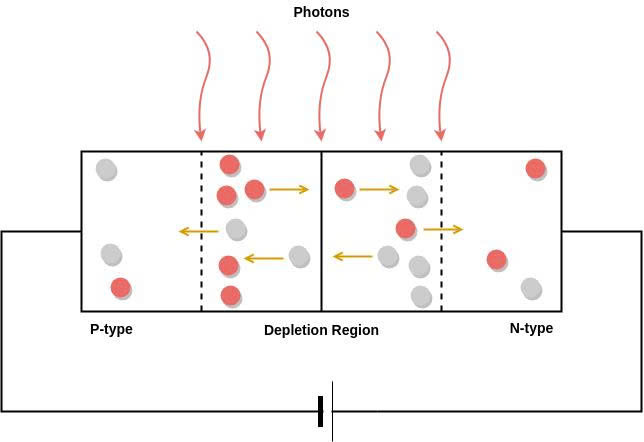
\includegraphics[width=0.7\textwidth]{picture/components/photo-diode.jpg}
    \caption{Linh kiện photo diode}
    \label{fig:component-photo-diode}
\end{figure}

Photo diode là linh kiện quang bán dẫn dùng để biến đổi tín hiệu ánh sáng thành tín hiệu điện, dựa trên hiệu ứng quang điện trong tiếp giáp p-n (hoặc cấu trúc PIN). Khi photon có năng lượng phù hợp đi vào vùng nghèo, các cặp electron--lỗ trống được sinh ra và tạo dòng quang tỉ lệ với cường độ chiếu sáng.

Trong nguyên lý làm việc, photo diode thường được phân cực ngược để mở rộng vùng nghèo, giảm điện dung tiếp giáp và tăng tốc độ đáp ứng. Ở chế độ này, dòng tối tồn tại khi không có ánh sáng; khi có ánh sáng chiếu vào, dòng quang tăng lên và được chuyển đổi thành điện áp qua điện trở tải hoặc mạch khuếch đại chuyển dòng-áp (TIA) để đưa vào kênh đo ADC.

Các thông số kỹ thuật cơ bản cần xem xét gồm: dải bước sóng đáp ứng, độ nhạy (A/W), dòng tối, điện dung tiếp giáp, thời gian đáp ứng, diện tích vùng nhạy quang, điện áp phân cực ngược tối đa và độ tuyến tính theo công suất sáng. Việc chọn đúng các tham số này giúp cải thiện tỉ số tín hiệu trên nhiễu và độ chính xác của hệ đo quang.

Với photo diode, quan hệ cơ bản giữa công suất ánh sáng tới và dòng quang sinh ra được mô tả bởi:
\begin{equation}
I_{ph} = R_{\lambda} P_{opt}
\end{equation}

Trong đó, hệ số đáp ứng quang theo bước sóng có thể viết:
\begin{equation}
R_{\lambda} = \eta \frac{q\lambda}{hc}
\end{equation}

Nếu nguồn sáng gần đơn sắc và công suất tới gần như không đổi trong thời gian \(t\), có thể liên hệ thêm giữa năng lượng ánh sáng tới và điện lượng quang sinh ra:
\begin{equation}
Q_{ph} = I_{ph} t = R_{\lambda} E_{opt}
\end{equation}

Trong đó:
\begin{itemize}
    \item \(I_{ph}\) là dòng quang sinh ra bởi photo diode, đơn vị A. Đây là thành phần dòng do ánh sáng gây ra, chưa kể đến dòng tối của linh kiện.
    \item \(R_{\lambda}\) là độ nhạy hay responsivity của photo diode tại bước sóng \(\lambda\), đơn vị A/W. Tham số này cho biết với mỗi watt công suất quang tới ở bước sóng xác định, photo diode tạo ra bao nhiêu ampere dòng quang.
    \item \(P_{opt}\) là công suất quang tới bề mặt nhạy sáng của photo diode, đơn vị W. Đây là công suất quang thực sự đi vào vùng nhạy quang, không phải toàn bộ công suất phát của nguồn nếu trên đường truyền còn có suy hao.
    \item \(\eta\) là hiệu suất lượng tử của photo diode, không có đơn vị. Đại lượng này biểu diễn tỉ lệ giữa số hạt tải điện hữu ích được tạo ra và số photon tới vùng nhạy quang.
    \item \(q\) là điện tích electron, xấp xỉ \(1.602\times10^{-19}\,C\). Đây là điện lượng cơ bản gắn với mỗi hạt tải điện được thu gom.
    \item \(\lambda\) là bước sóng ánh sáng tới, đơn vị m. Giá trị này ảnh hưởng trực tiếp đến năng lượng của từng photon và do đó ảnh hưởng đến responsivity của linh kiện.
    \item \(h\) là hằng số Planck, xấp xỉ \(6.626\times10^{-34}\,J\cdot s\).
    \item \(c\) là tốc độ ánh sáng trong chân không, xấp xỉ \(3\times10^8\,m/s\).
    \item \(Q_{ph}\) là điện lượng quang thu được trong thời gian quan sát, đơn vị C.
    \item \(E_{opt}\) là năng lượng ánh sáng tới photo diode trong khoảng thời gian xét, đơn vị J.
    \item \(t\) là thời gian chiếu sáng hoặc thời gian lấy mẫu, đơn vị s.
\end{itemize}

Các biểu thức trên cho thấy photo diode thực hiện quá trình biến đổi theo chuỗi: năng lượng ánh sáng tới quyết định công suất quang tới, công suất quang tới cùng với bước sóng xác định responsivity, và responsivity quyết định dòng quang đầu ra. Vì vậy, khi tính toán hệ đo quang, cần đặc biệt chú ý đến bước sóng \(\lambda\), độ nhạy \(R_{\lambda}\), suy hao trên đường truyền quang và thời gian lấy mẫu để dự đoán chính xác mức dòng điện thu được ở đầu vào mạch khuếch đại hoặc ADC.



\newpage

